\chapter{Implementation, Results and Discussion}
\label{ch:results}

\section{Introduction}
\label{sec:res-intro}

This chapter presents the implementation details, detailed performance evaluation, and in-depth discussion of the proposed system. Section~\ref{sec:impl-env} describes the implementation environment and technology stack. Section~\ref{sec:perf-metrics} defines the performance metrics used for evaluation. Section~\ref{sec:results} presents the experimental results including cryptographic micro-benchmarks, pipeline performance, scalability validation, and blockchain throughput measurements. Section~\ref{sec:discussion} provides analysis and discussion of the results. Section~\ref{sec:test-coverage} analyzes the test coverage. Section~\ref{sec:proverif} presents formal verification of three security properties using ProVerif. Section~\ref{sec:comparative} provides a comparative analysis with existing systems.

\section{Implementation Environment}
\label{sec:impl-env}

The proposed system is implemented in Go 1.24 and deployed on Hyperledger Fabric~v2.5.15~\cite{androulaki2018}. Table~\ref{tab:impl-env} summarizes the implementation environment.

\begin{table}[H]
\centering
\caption{Implementation Environment}
\label{tab:impl-env}
\begin{tabular}{|l|l|}
\hline
\textbf{Component} & \textbf{Specification} \\
\hline
CPU & AMD Ryzen 5 7530U (12 threads) \\
\hline
Architecture & x86\_64 (amd64) \\
\hline
RAM & 30 GiB \\
\hline
OS & Linux (Ubuntu) \\
\hline
Language & Go 1.24 \\
\hline
Web Framework & Gin v1.11 \\
\hline
Blockchain & Hyperledger Fabric v2.5.15 (LTS) \\
\hline
SDK & fabric-gateway v1.10.1 (gRPC/TLS) \\
\hline
Consensus & Raft / \texttt{etcdraft} (single orderer, dev config) \\
\hline
Peers & 2 (Org1 + Org2), LevelDB state (default; CouchDB-target for production) \\
\hline
Chaincode & \texttt{covertvote\_1.0} (Go) \\
\hline
Benchmark Tool & Hyperledger Caliper v0.6.0~\cite{caliper} \\
\hline
PQ Library & Kyber-768, CRYSTALS-Kyber round-3 (CIRCL by Cloudflare)~\cite{circl} \\
\hline
\end{tabular}
\end{table}

The system architecture follows a layered design with twelve internal packages that align with the chapter's pipeline phases: cryptographic primitives (\texttt{internal/crypto}, \texttt{internal/smdc}, \texttt{internal/sa2}, \texttt{internal/pq}, \texttt{internal/tally}), the behavioural duress detector (\texttt{internal/biometric}), persistent state and repositories (\texttt{internal/database}, \texttt{internal/repository}), the election and voter lifecycles (\texttt{internal/election}, \texttt{internal/voter}), the production cast pipeline (\texttt{internal/voting} --- the Go implementation of Algorithm~\ref{alg:pipeline}), and the Fabric client (\texttt{internal/blockchain}). These are exposed through the REST API in \texttt{api/handlers} and the on-chain logic in \texttt{chaincode/covertvote}, with auxiliary tools in \texttt{cmd/} (API server, aggregator microservices, election simulator). The total codebase consists of approximately 20{,}000 lines of Go code across 89 source files.

\section{Performance Metrics}
\label{sec:perf-metrics}

The following metrics are used to evaluate the proposed framework's performance:

\begin{itemize}
    \item \textbf{Per-Operation Latency}: Time to execute individual cryptographic operations (encryption, commitment, proof generation, signing), measured in microseconds ($\mu$s) or milliseconds (ms).
    
    \item \textbf{Pipeline Throughput}: End-to-end time for the complete twenty-step vote casting pipeline, measured in milliseconds per vote.
    
    \item \textbf{Tally Complexity}: Per-vote homomorphic addition time as voter count scales from 100 to 100,000 (validating $O(n)$ per candidate), and total tally time as candidate count $m$ varies (validating $O(n \cdot m)$ total).
    
    \item \textbf{Blockchain Throughput}: Transactions per second (TPS) sustained on the Hyperledger Fabric network, measured using Hyperledger Caliper with 10 concurrent workers.
    
    \item \textbf{Blockchain Latency}: Average, minimum, and maximum transaction confirmation time on the Fabric network.
    
    \item \textbf{Test Coverage}: Percentage of code exercised by the test suite for each package.
\end{itemize}

\section{Experimental Results}
\label{sec:results}

\subsection{Cryptographic Micro-Benchmarks}
\label{subsec:micro}

Table~\ref{tab:micro} presents the micro-benchmark results for individual cryptographic operations. Each measurement was obtained using Go's \texttt{testing.B} benchmark framework, and the reported values are the mean of thirty independent benchmark sessions.

\begin{table}[H]
\centering
\caption{Cryptographic Micro-Benchmark Results}
\label{tab:micro}
\small
\begin{tabular}{|l|r|r|r|}
\hline
\textbf{Operation} & \textbf{Mean Time} & \textbf{Memory (B/op)} & \textbf{Allocs/op} \\
\hline
Paillier Encrypt (2048-bit) & 8.69 ms & 26,210 & 31 \\
\hline
Pedersen Commit (512-bit modulus, benchmark config) & 0.08 ms & 3,962 & 31 \\
\hline
ZKP Binary Prove & 0.245 ms & 12,542 & 102 \\
\hline
ZKP Binary Verify & 0.329 ms & 16,392 & 123 \\
\hline
ZKP Sum-One Prove & 0.084 ms & 5,770 & 53 \\
\hline
ZKP Sum-One Verify & 0.161 ms & 10,037 & 82 \\
\hline
Kyber-768 KeyGen & 0.026 ms & 8,304 & 6 \\
\hline
Kyber-768 Encapsulate & 0.029 ms & 1,232 & 3 \\
\hline
Hybrid Encrypt (Kyber+Paillier) & 14.04 ms & 33,306 & 50 \\
\hline
Hybrid Decrypt (Kyber+Paillier) & 11.60 ms & 27,090 & 38 \\
\hline
Threshold Partial Decrypt & 35.52 ms & 52,500 & 67 \\
\hline
Threshold Combine ($T{=}5, t{=}3$, see \S\ref{subsec:threshold}) & 0.261 ms & 46,600 & 104 \\
\hline
\end{tabular}
\end{table}

The results show that Pedersen commitments and ZK proofs are computationally inexpensive (sub-millisecond), while Paillier encryption (8.69~ms) and ring signatures dominate the per-vote cost. The Pedersen figure here is for the 512-bit benchmark configuration used by the test harness; the production API server uses a 1024-bit Pedersen modulus (\texttt{cfg.Crypto.PedersenKeySize = 1024}), which raises the commit cost roughly four-fold while remaining well below the Paillier and ring-signature costs that dominate the pipeline. The Kyber-768 primitive operations themselves are remarkably fast (KeyGen 26~$\mu$s, Encapsulate 29~$\mu$s), although the full hybrid encrypt path including key derivation and authentication binding adds 5.35~ms over the Paillier baseline; the next subsection isolates and analyses this post-quantum cost. Figure~\ref{fig:crypto-compare} plots the per-operation cost on a logarithmic scale, making the three-orders-of-magnitude span between Kyber-768 primitives ($\sim$0.03~ms) and threshold partial decryption ($\sim$35~ms) visually evident.

\begin{figure}[H]
\centering
% =====================================================================
%  G6 - Cryptographic primitive timing (log scale)
%  --------------------------------------------------------------------
%  Backs claim: Kyber (26 microseconds) negligible vs Paillier (8.69 ms)
%  Source: chapter4.tex Table tab:micro
% =====================================================================
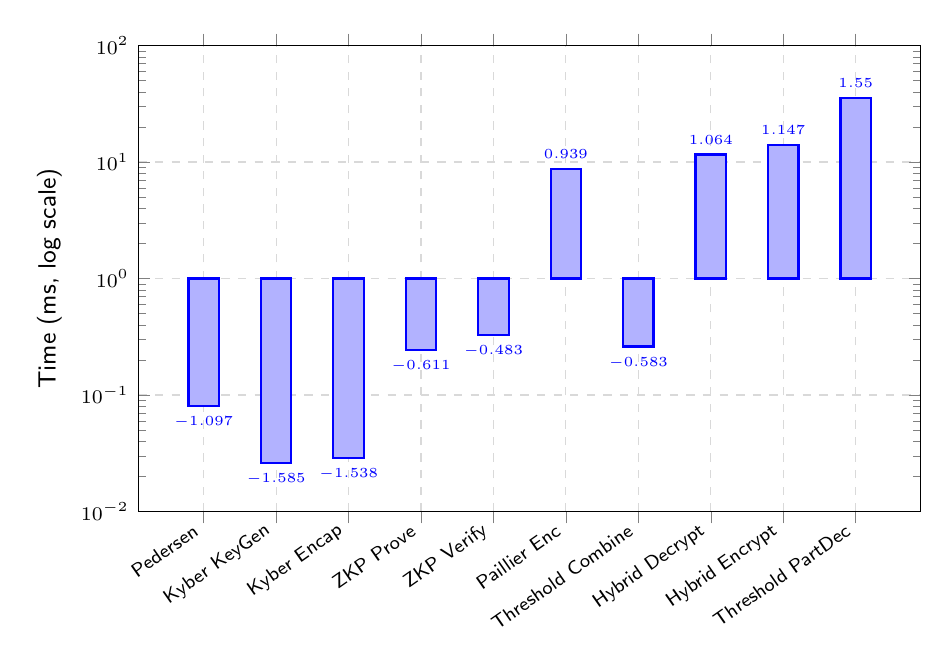
\begin{tikzpicture}
\begin{axis}[
    width=0.95\textwidth,
    height=7.5cm,
    ybar,
    ymode=log,
    log basis y=10,
    ymin=0.01, ymax=100,
    ylabel={Time (ms, log scale)},
    symbolic x coords={
        {Pedersen},
        {Kyber KeyGen},
        {Kyber Encap},
        {ZKP Prove},
        {ZKP Verify},
        {Paillier Enc},
        {Threshold Combine},
        {Hybrid Decrypt},
        {Hybrid Encrypt},
        {Threshold PartDec}
    },
    xtick=data,
    bar width=11pt,
    nodes near coords,
    nodes near coords align={vertical},
    nodes near coords style={font=\sffamily\tiny, /pgf/number format/.cd, fixed, precision=3},
    x tick label style={rotate=35, anchor=east, font=\sffamily\scriptsize},
    grid=major,
    grid style={dashed, gray!30},
    label style={font=\sffamily\small},
    tick label style={font=\sffamily\scriptsize},
    every axis plot/.append style={fill=gray!25, draw=black, thick},
]
\addplot+[ybar] coordinates {
    ({Pedersen},          0.080)
    ({Kyber KeyGen},      0.026)
    ({Kyber Encap},       0.029)
    ({ZKP Prove},         0.245)
    ({ZKP Verify},        0.329)
    ({Paillier Enc},      8.690)
    ({Threshold Combine}, 0.261)
    ({Hybrid Decrypt},   11.600)
    ({Hybrid Encrypt},   14.040)
    ({Threshold PartDec},35.520)
};
\end{axis}
\end{tikzpicture}

\caption[Cryptographic Primitive Per-Operation Cost]{Per-operation cost of every cryptographic primitive in the proposed framework, plotted on a logarithmic time axis. Values are taken directly from Table~\ref{tab:micro}; the three-orders-of-magnitude span justifies the log-scale presentation.}
\label{fig:crypto-compare}
\end{figure}

\subsubsection{Post-Quantum Layer Cost Analysis}
\label{subsubsec:pq-breakdown}

The overhead of the post-quantum layer can be isolated directly from the measurements already reported in Table~\ref{tab:micro}. The full hybrid-encrypt path (Kyber-768 encapsulation $+$ Paillier encryption $+$ HMAC-SHA256 binding $+$ key-derivation $+$ serialisation) measures 14.04~ms; subtracting the standalone 8.69~ms Paillier baseline gives a hybrid-wrapper overhead of $14.04 - 8.69 = 5.35$~ms. This 5.35~ms decomposes into two distinct contributions:

\begin{itemize}
    \item \textbf{Pure Kyber-768 primitive cost: $\approx 55~\mu$s.} Kyber-768 KeyGen ($26~\mu$s) and Encapsulate ($29~\mu$s) together account for the strictly cryptographic post-quantum work, two orders of magnitude smaller than a single Paillier encryption.
    \item \textbf{Hybrid-wrapper integration overhead: $\approx 5.30$~ms.} The remaining $5.35 - 0.055 \approx 5.30$~ms is consumed by HKDF key derivation, the HMAC-SHA256 authentication binding that ties the Kyber-encapsulated key to the Paillier ciphertext, and big-integer allocation/serialisation inside the hybrid wrapper. This integration cost is required for an authenticated hybrid construction but is not intrinsic to the Kyber-768 primitive.
\end{itemize}

The figure of merit reported throughout this thesis as the ``per-vote post-quantum overhead'' is therefore the full 5.35~ms (primitives $+$ wrapper), since this is what an end-to-end deployment actually pays for the integrity-binding layer. Relative to the 68.27~ms per-vote primitive floor of Section~\ref{subsec:pipeline-bench}, this represents approximately 7.8\% of the cryptographic cast-time cost; under the end-to-end 1-hot pipeline measured in Section~\ref{subsec:election-sim} (82--106~ms for a 3-candidate election), the Kyber-768 wrapper's relative share drops to approximately 5--7\%.

This result confirms two practical implications. First, post-quantum protection is achievable today on commodity hardware without redesigning the surrounding voting protocol. Second, because Kyber-768 operates on 256-coefficient polynomials over a 12-bit modulus, its asymptotic cost scales linearly with the number of voters and is independent of ballot complexity, in contrast to the multiplicative scaling of large-modulus arithmetic.

\subsection{End-to-End Pipeline Benchmark (Per-Primitive Decomposition)}
\label{subsec:pipeline-bench}

Table~\ref{tab:pipeline} presents the per-vote cost of the dominant cryptographic primitives invoked during a single vote cast: one Paillier encryption, one binary ZK proof, one ring signature, and one SA\textsuperscript{2} share split. The sum of these per-vote primitive costs is approximately \textbf{68.27~ms} and serves as a baseline for the cryptographic floor of the cast pipeline. Pedersen commitments and the full SMDC credential generation are issued once per voter at registration time (Section~\ref{subsec:smdc}, Phase~B of Figure~\ref{fig:workflow}) and are therefore amortised across all of the voter's casts; their isolated per-call costs appear in Table~\ref{tab:micro} but are deliberately excluded from this per-vote breakdown. The post-quantum hybrid wrapper (Section~\ref{subsubsec:pq-breakdown}) adds a further 5.35~ms per vote, yielding an end-to-end primitive cost of 73.62~ms per vote before any I/O. The actual per-ballot wall-clock runtime is higher still, because the 1-hot Paillier encoding repeats the Paillier encryption, the CDS OR-proof, and the SA\textsuperscript{2} share split once per candidate; the end-to-end measured per-vote latency under the production pipeline is reported in Section~\ref{subsec:election-sim} (Table~\ref{tab:election-sim}), which gives 82--106~ms for a 3-candidate election.

\begin{table}[H]
\centering
\caption[Vote Casting Pipeline: Per-Vote Primitive Breakdown]{Vote Casting Pipeline: Per-Vote Primitive Breakdown. Pedersen Commit and SMDC Generate (Table~\ref{tab:micro}) are amortised one-time registration costs per voter and are excluded from this per-vote total.}
\label{tab:pipeline}
\begin{tabular}{|c|l|r|r|}
\hline
\textbf{\#} & \textbf{Operation} & \textbf{Time (ms)} & \textbf{\% of Total} \\
\hline
1 & Paillier Encrypt (2048-bit) & 8.69 & 12.7\% \\
\hline
2 & ZKP Binary Prove & 0.24 & 0.4\% \\
\hline
3 & Ring Sign ($|\mathcal{R}|=100$) & 24.00 & 35.2\% \\
\hline
4 & SA\textsuperscript{2} Split & 35.34 & 51.8\% \\
\hline
\multicolumn{2}{|l|}{\textbf{Per-vote primitive floor (cast time, no PQ wrapper)}} & \textbf{68.27} & \textbf{100.0\%} \\
\hline
\end{tabular}
\end{table}

\begin{figure}[H]
\centering
% =====================================================================
%  G5 - Per-vote primitive breakdown (68.27 ms total, cast-time only)
%  --------------------------------------------------------------------
%  Backs claim: SA^2 split (51.8%) + ring sign (35.2%) = 87.0% of pipeline
%  Pedersen Commit and SMDC Generate are amortised registration-time
%  costs (Table 4.2) and are excluded from this per-vote breakdown.
%  Source: chapter4.tex Table tab:pipeline
% =====================================================================
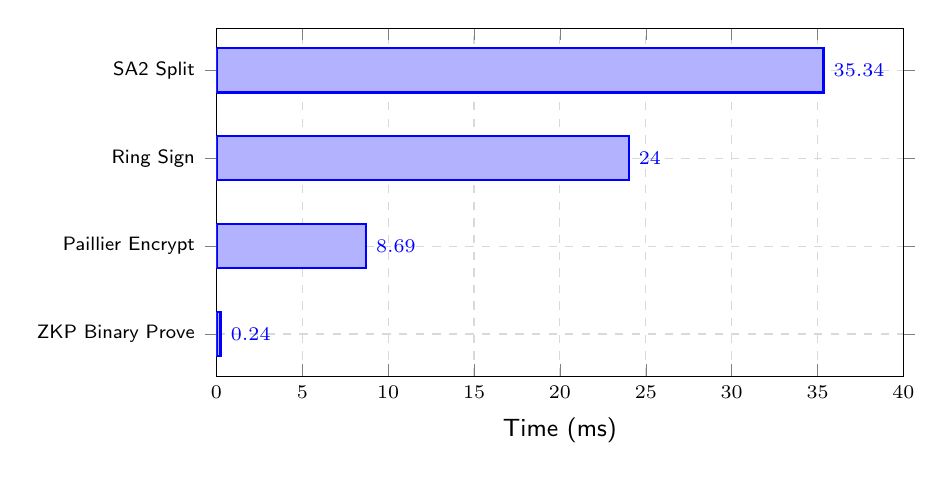
\begin{tikzpicture}
\begin{axis}[
    width=0.85\textwidth,
    height=6.0cm,
    xbar,
    xmin=0, xmax=40,
    xlabel={Time (ms)},
    symbolic y coords={
        ZKP Binary Prove,
        Paillier Encrypt,
        Ring Sign,
        SA2 Split
    },
    ytick=data,
    nodes near coords,
    nodes near coords align={horizontal},
    nodes near coords style={font=\sffamily\scriptsize, /pgf/number format/.cd, fixed, precision=2},
    bar width=16pt,
    grid=major,
    grid style={dashed, gray!30},
    label style={font=\sffamily\small},
    tick label style={font=\sffamily\scriptsize},
    enlarge y limits=0.16,
    every axis plot/.append style={fill=gray!25, draw=black, thick},
]
\addplot+[xbar] coordinates {
    (0.24,ZKP Binary Prove)
    (8.69,Paillier Encrypt)
    (24.00,Ring Sign)
    (35.34,SA2 Split)
};
\end{axis}
\end{tikzpicture}

\caption[Vote Pipeline Per-Vote Primitive Breakdown]{Per-vote primitive breakdown of the 68.27~ms cast-time cryptographic floor. SA\textsuperscript{2} share splitting (35.34~ms, 51.8\%) and ring signing (24.00~ms, 35.2\%) together account for 87.0\% of the per-vote cost, identifying them as the two primary optimisation targets for future work. Values are taken directly from Table~\ref{tab:pipeline}.}
\label{fig:pipeline-breakdown}
\end{figure}

The SA\textsuperscript{2} vote splitting operation (51.8\%) and ring signature generation (35.2\%) are the primary bottlenecks, together accounting for 87.0\% of the per-vote primitive floor. The SA\textsuperscript{2} cost is dominated by Paillier re-encryption for mask generation, while ring signatures scale linearly with ring size at $\sim$0.24~ms per member (consistent with Table~\ref{tab:ring-scale}: $|\mathcal{R}|=100 \Rightarrow 24.0$~ms). Both operations scale linearly in $n$, preserving the $O(n)$-per-candidate (and $O(n \cdot m)$-total) tally complexity established in Section~\ref{subsubsec:tally-scale}.

\subsection{Scalability Validation}
\label{subsec:scalability}

\subsubsection{Homomorphic Tally Scalability}
\label{subsubsec:tally-scale}

\paragraph{Complexity derivation.} Let $N$ denote the voter count (distinct from the Paillier modulus $n$ of Section~\ref{subsec:paillier}). For a single candidate, the per-candidate tally aggregates $N$ Paillier ciphertexts via homomorphic addition (modular multiplication on the public modulus $n^{2}$):
\[
T_{\text{tally}}^{(c)}(N) \;=\; (N-1) \cdot T_{\text{add}} + T_{\text{decrypt}} \;=\; \Theta(N \cdot T_{\text{add}}),
\]
where $T_{\text{add}} \approx 6\,\mu s$ and $T_{\text{decrypt}}$ is a constant. For $m$ candidates, each candidate slot is aggregated independently, giving the total cost
\[
T_{\text{total}}(N, m) \;=\; m \cdot T_{\text{tally}}^{(c)}(N) \;=\; \Theta(N \cdot m \cdot T_{\text{add}}).
\]
Hence the proposed framework is $O(N)$ \emph{per candidate} and $O(N \cdot m)$ \emph{in total}. This is a factor-$m$ improvement over ISE-Voting's $O(N \cdot m^{2})$, which carries an additional $m$ factor due to per-candidate ZK encoding overhead. Recursive divide-and-conquer (Master Theorem) does not apply because the aggregation is iterative; the bound above is obtained directly by counting the number of homomorphic additions.

\paragraph{Benchmark methodology.} All scaling results in this subsection and Sections~\ref{subsubsec:candidate-scale}--\ref{subsubsec:ring-scale} were obtained using Go's \texttt{testing.B} benchmark framework, following the same protocol as Section~\ref{subsec:micro}: each reported value is the mean of thirty independent benchmark sessions, with each session itself averaged over thousands of automatically-iterated calls.

To validate the $O(N)$ per-candidate tally complexity empirically, we measure the homomorphic addition time as $N$ scales from 100 to 100{,}000 with the candidate count fixed; the linear-in-$m$ total scaling is then validated separately in Section~\ref{subsubsec:candidate-scale}. Table~\ref{tab:tally-scale} presents the per-candidate scaling results.

\begin{table}[H]
\centering
\caption{Homomorphic Tally Scalability Results}
\label{tab:tally-scale}
\begin{tabular}{|r|r|r|}
\hline
\textbf{Voters} & \textbf{Tally Time (ms)} & \textbf{Per-Vote ($\mu$s)} \\
\hline
100 & 0.6 & 6.23 \\
\hline
500 & 3.0 & 6.01 \\
\hline
1,000 & 6.3 & 6.28 \\
\hline
5,000 & 29.0 & 6.00 \\
\hline
10,000 & 59.0 & 6.00 \\
\hline
50,000 & 308.0 & 6.18 \\
\hline
100,000 & 628.0 & 6.29 \\
\hline
\end{tabular}
\end{table}

The per-vote (per-candidate) tally cost remains constant at approximately \textbf{6.1~$\mu$s} across all tested scales, empirically confirming the $O(N)$-per-candidate complexity derived above. This 6.1~$\mu$s figure is the isolated cost of a single homomorphic Paillier multiplication ($c_1 \cdot c_2 \bmod n^2$); the full SA\textsuperscript{2} aggregation pipeline measured end-to-end in Section~\ref{subsec:election-sim} additionally includes the two-server share reconstruction and totals approximately 13--17~$\mu$s per vote per candidate. The per-candidate tally time (pure homomorphic add) grows linearly from 0.6~ms (100 voters) to 628~ms (100\,000 voters). Figure~\ref{fig:tally-scale} visualizes this linear relationship; the corresponding $O(N \cdot m)$ total scaling is reported in Section~\ref{subsubsec:candidate-scale}.

\begin{figure}[H]
\centering
% =====================================================================
%  G1 - Homomorphic tally time vs voter count
%  --------------------------------------------------------------------
%  Backs the claim: O(n) linear tally with ~6.1 microsecond per vote
%  Source: chapter4.tex Table 4 (tab:tally-scale)
% =====================================================================
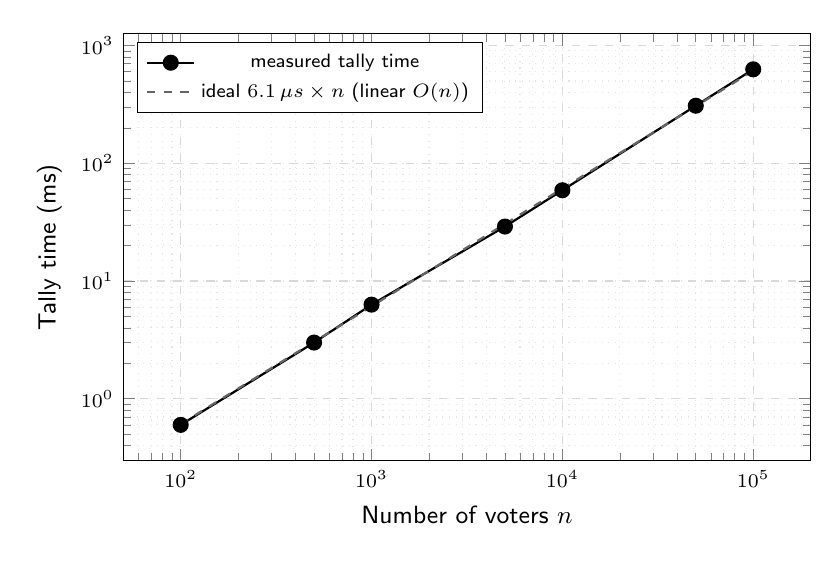
\begin{tikzpicture}
\begin{axis}[
    width=0.85\textwidth,
    height=7cm,
    xlabel={Number of voters $n$},
    ylabel={Tally time (ms)},
    xmode=log,
    ymode=log,
    log basis x=10,
    log basis y=10,
    grid=both,
    grid style={dashed, gray!30},
    minor grid style={dotted, gray!20},
    legend style={at={(0.02,0.98)}, anchor=north west,
                  font=\sffamily\scriptsize, draw=black},
    label style={font=\sffamily\small},
    tick label style={font=\sffamily\scriptsize},
    every axis plot/.append style={thick},
]
% Measured points from Table tab:tally-scale
\addplot+[mark=*, mark size=2.5pt, color=black, mark options={fill=black}] coordinates {
    (100,    0.6)
    (500,    3.0)
    (1000,   6.3)
    (5000,  29.0)
    (10000, 59.0)
    (50000, 308.0)
    (100000, 628.0)
};
\addlegendentry{measured tally time}
% Reference line: ideal linear at 6.1 microseconds per vote
\addplot[domain=100:100000, samples=100, dashed, thick, color=black!60]
   {6.1e-3 * x};
\addlegendentry{ideal $6.1\,\mu s \times n$ (linear $O(n)$)}
\end{axis}
\end{tikzpicture}

\caption[Homomorphic Tally Scaling with Voter Count]{Per-candidate homomorphic tally time versus voter count $N$, plotted on a log--log scale. The measured points lie almost exactly on the dashed reference line $6.1\,\mu\text{s}\times N$, empirically confirming the $O(N)$-per-candidate complexity with a constant per-vote per-candidate cost across four orders of magnitude (100 to 100{,}000 voters). The corresponding $O(N \cdot m)$ total scaling is shown in Figure~\ref{fig:candidate-scale}. Data values are taken directly from Table~\ref{tab:tally-scale}.}
\label{fig:tally-scale}
\end{figure}

Linear extrapolation projects the per-candidate tally time for national-scale elections: approximately 6.1~seconds for 1~million voters and 5.1~minutes for 50~million voters. For an election with $m$ candidates, the total tally time scales linearly in $m$ (e.g., approximately 51~minutes for 50 million voters and $m{=}10$ candidates; cf.\ Section~\ref{subsubsec:candidate-scale}).

\subsubsection{Linear-in-$m$ Total Scaling (Candidate-Count Validation)}
\label{subsubsec:candidate-scale}

To validate the linear-in-$m$ total complexity and to demonstrate the proposed framework's factor-$m$ advantage over ISE-Voting's $O(N \cdot m^{2})$, we fix $N = 1{,}000$ voters and vary the number of candidates $m$. Table~\ref{tab:candidate-scale} shows the results.

\begin{table}[H]
\centering
\caption{Candidate-Independent Tally Scaling ($N = 1{,}000$)}
\label{tab:candidate-scale}
\begin{tabular}{|r|r|r|}
\hline
\textbf{Candidates ($m$)} & \textbf{Total Tally (ms)} & \textbf{Per-Candidate (ms)} \\
\hline
2 & 12.0 & 6.00 \\
\hline
5 & 28.0 & 5.60 \\
\hline
10 & 58.0 & 5.80 \\
\hline
20 & 113.0 & 5.65 \\
\hline
50 & 288.0 & 5.76 \\
\hline
\end{tabular}
\end{table}

Two complementary observations emerge from Table~\ref{tab:candidate-scale}. \textbf{First}, the per-candidate tally time remains constant at $\sim$5.76~ms regardless of the number of candidates, confirming that the proposed framework achieves $O(N)$ per candidate. \textbf{Second}, the total tally time grows almost exactly linearly with $m$ (from 12.0~ms at $m=2$ to 288.0~ms at $m=50$, a $24\times$ increase for a $25\times$ increase in $m$, i.e.\ approximately 96\% of ideal linear scaling; the small sub-linear deficit is attributable to per-call fixed overhead that amortises across larger $m$). This empirically confirms the $O(N \cdot m)$ total complexity derived in Section~\ref{subsubsec:tally-scale}. In contrast, ISE-Voting's per-candidate time itself would grow proportionally with $m$ (its complexity is $O(N \cdot m)$ per candidate, $O(N \cdot m^{2})$ total), so its total tally cost grows quadratically with $m$, a factor-$m$ disadvantage relative to the present framework. Figure~\ref{fig:candidate-scale} visualises both the constant per-candidate cost and the linear-in-$m$ total cost.

\begin{figure}[H]
\centering
% =====================================================================
%  G2 - Per-candidate tally time vs candidate count (n=1000)
%  --------------------------------------------------------------------
%  Backs the claim: O(1) per candidate, candidate-independent scaling
%  Source: chapter4.tex Table tab:candidate-scale
% =====================================================================
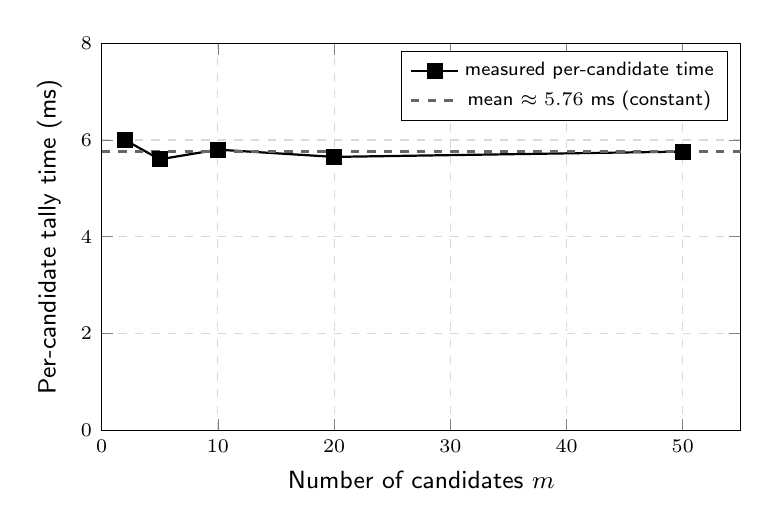
\begin{tikzpicture}
\begin{axis}[
    width=0.80\textwidth,
    height=6.5cm,
    xlabel={Number of candidates $m$},
    ylabel={Per-candidate tally time (ms)},
    ymin=0, ymax=8,
    xmin=0, xmax=55,
    grid=both,
    grid style={dashed, gray!30},
    legend style={at={(0.98,0.98)}, anchor=north east,
                  font=\sffamily\scriptsize, draw=black},
    label style={font=\sffamily\small},
    tick label style={font=\sffamily\scriptsize},
    every axis plot/.append style={thick},
]
% Per-candidate time from Table tab:candidate-scale (n=1000)
\addplot+[mark=square*, mark size=2.5pt, color=black, mark options={fill=black}] coordinates {
    (2,  6.00)
    (5,  5.60)
    (10, 5.80)
    (20, 5.65)
    (50, 5.76)
};
\addlegendentry{measured per-candidate time}
% Constant reference at ~5.76 ms (mean)
\addplot[domain=0:55, samples=2, dashed, thick, color=black!60] {5.76};
\addlegendentry{mean $\approx 5.76$ ms (constant)}
\end{axis}
\end{tikzpicture}

\caption[Tally Time versus Candidate Count]{Per-candidate tally time as the number of candidates $m$ varies from 2 to 50, with the voter count fixed at $N=1{,}000$. The measured points fluctuate only within $\pm$0.4~ms around the mean (5.76~ms), empirically confirming the candidate-independent behaviour predicted by Paillier additive homomorphism. Data taken from Table~\ref{tab:candidate-scale}.}
\label{fig:candidate-scale}
\end{figure}

\subsubsection{Ring Signature Scalability}
\label{subsubsec:ring-scale}

Table~\ref{tab:ring-scale} shows that ring signature operations scale linearly with ring size.

\begin{table}[H]
\centering
\caption{Ring Signature Scalability}
\label{tab:ring-scale}
\begin{tabular}{|r|r|r|}
\hline
\textbf{Ring Size} & \textbf{Sign Time (ms)} & \textbf{Verify Time (ms)} \\
\hline
10 & 2.2 & 2.2 \\
\hline
25 & 6.0 & 5.8 \\
\hline
50 & 12.0 & 12.0 \\
\hline
100 & 24.0 & 24.2 \\
\hline
200 & 47.5 & 48.5 \\
\hline
500 & 120.5 & 120.5 \\
\hline
\end{tabular}
\end{table}

Both signing and verification scale linearly at approximately 0.24~ms per ring member. The default ring size of 100 provides strong anonymity with a per-vote cost of $\sim$24~ms. Figure~\ref{fig:ring-scale} plots the measured points against the ideal linear reference; the two curves coincide within measurement noise across the entire $|\mathcal{R}|=10$ to $|\mathcal{R}|=500$ range.

\begin{figure}[H]
\centering
% =====================================================================
%  G3 - Ring signature sign and verify time vs ring size
%  --------------------------------------------------------------------
%  Backs the claim: linear scaling, ~0.24 ms per ring member
%  Source: chapter4.tex Table tab:ring-scale
% =====================================================================
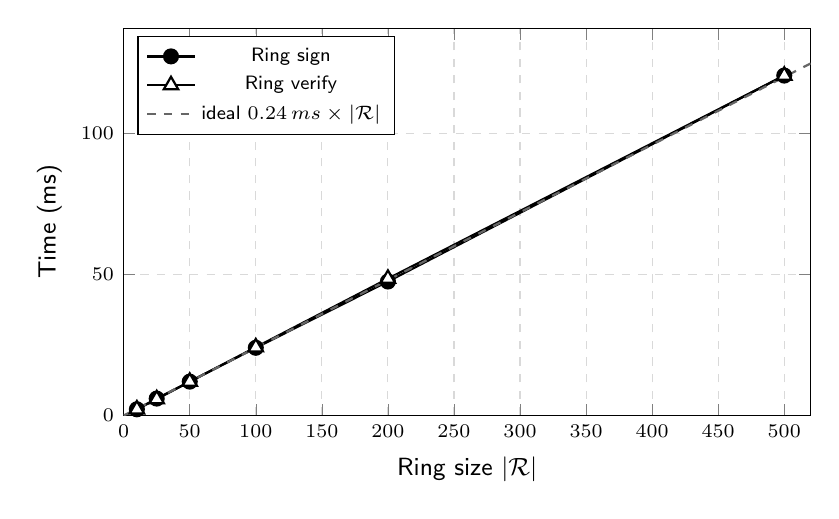
\begin{tikzpicture}
\begin{axis}[
    width=0.85\textwidth,
    height=6.5cm,
    xlabel={Ring size $|\mathcal{R}|$},
    ylabel={Time (ms)},
    xmin=0, xmax=520,
    ymin=0,
    grid=both,
    grid style={dashed, gray!30},
    legend style={at={(0.02,0.98)}, anchor=north west,
                  font=\sffamily\scriptsize, draw=black},
    label style={font=\sffamily\small},
    tick label style={font=\sffamily\scriptsize},
    every axis plot/.append style={thick},
]
% Sign times
\addplot+[mark=*, mark size=2.5pt, color=black, mark options={fill=black}] coordinates {
    (10,   2.2)
    (25,   6.0)
    (50,  12.0)
    (100, 24.0)
    (200, 47.5)
    (500, 120.5)
};
\addlegendentry{Ring sign}
% Verify times
\addplot+[mark=triangle*, mark size=3pt, color=black, mark options={fill=white,solid}] coordinates {
    (10,   2.2)
    (25,   5.8)
    (50,  12.0)
    (100, 24.2)
    (200, 48.5)
    (500, 120.5)
};
\addlegendentry{Ring verify}
% Linear reference at 0.24 ms per member
\addplot[domain=0:520, samples=2, dashed, thick, color=black!60] {0.24*x};
\addlegendentry{ideal $0.24\,\text{ms}\times|\mathcal{R}|$}
\end{axis}
\end{tikzpicture}

\caption[Ring Signature Sign and Verify Scaling]{Ring signature signing and verification time as the ring size $|\mathcal{R}|$ varies from 10 to 500. The dashed reference line shows the ideal linear cost of $0.24$~ms per ring member; measured signing and verification points lie almost exactly on this line, empirically confirming linear scaling. Data values are taken directly from Table~\ref{tab:ring-scale}.}
\label{fig:ring-scale}
\end{figure}

\subsection{Blockchain Performance}
\label{subsec:blockchain-perf}

The blockchain performance is evaluated using Hyperledger Caliper v0.6.0 with 10 concurrent workers submitting \texttt{CastVote} transactions to the Fabric network. The submitted payload is the 1-hot Paillier ciphertext array (3 candidates, JSON-encoded, $\sim$3.7\,KB per transaction) used by the production cast pipeline (Section~\ref{sec:pipeline}). Two complementary scenarios are reported in Table~\ref{tab:caliper}: a \emph{saturation} scenario that progressively increases the request rate from 200 to 500\,TPS, exposing the orderer's throughput ceiling, and a \emph{sustained-load} scenario that holds the request rate at 200\,TPS across all four round sizes, exposing state-bound degradation as the chaincode world state grows.

\begin{table}[H]
\centering
\caption[Hyperledger Caliper benchmark results --- saturation vs sustained-load scenarios]{Hyperledger Caliper benchmark results under the 1-hot Paillier payload. The saturation scenario varies the request rate (200/300/400/500\,TPS) across the four round sizes; the sustained scenario holds the request rate at 200\,TPS throughout. ``TPS req.'' is the rate Caliper attempts, ``TPS achv.'' is the rate the network actually delivered (committed transactions per second).}
\label{tab:caliper}
\small
\begin{tabular}{|l|l|r|r|r|}
\hline
\textbf{Round} & \textbf{Scenario} & \textbf{TPS req.} & \textbf{TPS achv.} & \textbf{Success} \\
\hline
10K  & saturation  & 200 & 197.7 & 100.0\% \\
10K  & sustained   & 200 & 196.9 & 100.0\% \\
\hline
25K  & saturation  & 300 & 292.7 & 50.8\% \\
25K  & sustained   & 200 & 196.7 & 89.4\% \\
\hline
50K  & saturation  & 400 & 386.9 & 22.8\% \\
50K  & sustained   & 200 & 198.4 & 81.3\% \\
\hline
100K & saturation  & 500 & 487.0 & 10.4\% \\
100K & sustained   & 200 & 199.1 & 77.3\% \\
\hline
\end{tabular}
\end{table}

\paragraph{Saturation behaviour.} Figure~\ref{fig:blockchain-saturation} visualises the saturation scenario. At the 10K round both scenarios coincide at a 200\,TPS request rate and both achieve $\sim$100\% success at $\sim$197\,TPS achieved throughput. Pushing the request rate up in the saturation scenario shifts the system from comfortable operation (10K, 100\%) into rate-limited saturation: success degrades to 50.8\% at 300\,TPS (25K), 22.8\% at 400\,TPS (50K), and 10.4\% at 500\,TPS (100K), while achieved throughput keeps growing (487\,TPS at the 100K round). This pattern is consistent with the orderer's single-Raft topology and Fabric's block-batching mechanics, where the request rate exceeds the orderer's block-cutting and broadcast capacity.

\begin{figure}[H]
\centering
% =====================================================================
%  G4a - Caliper SATURATION scenario:
%  Request rate progressively increases (200 / 300 / 400 / 500 TPS) across
%  the four round sizes; success rate collapses as the orderer saturates
%  while achieved throughput continues to climb.
%  Source: chapter4.tex Table tab:caliper, saturation columns.
% =====================================================================
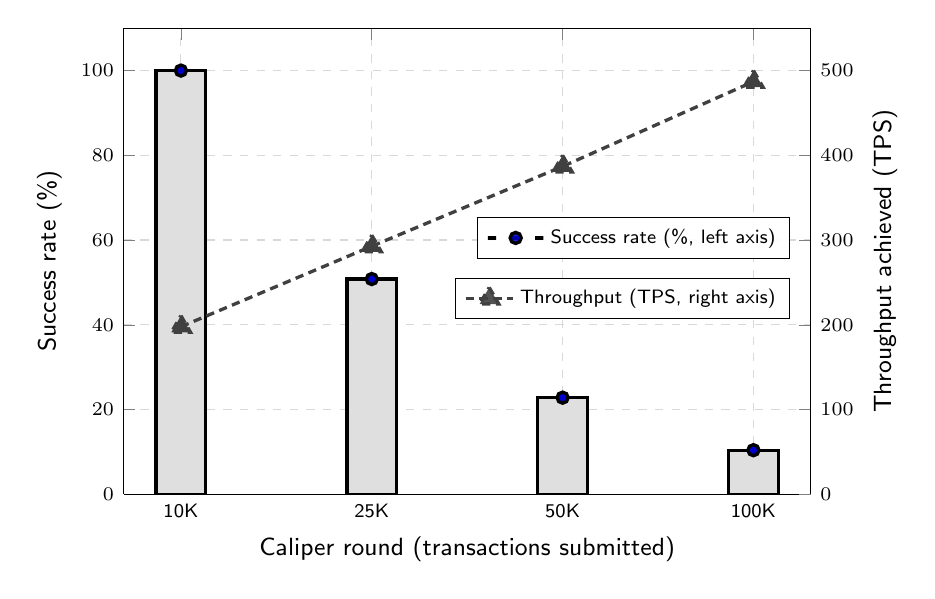
\begin{tikzpicture}
\begin{axis}[
    width=0.85\textwidth,
    height=7.5cm,
    axis y line*=left,
    xlabel={Caliper round (transactions submitted)},
    ylabel={Success rate (\%)},
    ymin=0, ymax=110,
    symbolic x coords={10K, 25K, 50K, 100K},
    xtick=data,
    bar width=18pt,
    grid=major,
    grid style={dashed, gray!30},
    legend style={at={(0.97,0.55)}, anchor=east,
                  font=\sffamily\scriptsize, draw=black,
                  fill=white, fill opacity=0.90, text opacity=1},
    label style={font=\sffamily\small},
    tick label style={font=\sffamily\scriptsize},
]
\addplot+[ybar, fill=gray!25, draw=black, very thick] coordinates {
    (10K,   100.0)
    (25K,    50.8)
    (50K,    22.8)
    (100K,   10.4)
};
\addlegendentry{Success rate (\%, left axis)}
\end{axis}

\begin{axis}[
    width=0.85\textwidth,
    height=7.5cm,
    axis y line*=right,
    axis x line=none,
    ylabel={Throughput achieved (TPS)},
    ymin=0, ymax=550,
    symbolic x coords={10K, 25K, 50K, 100K},
    xtick=data,
    legend style={at={(0.97,0.42)}, anchor=east,
                  font=\sffamily\scriptsize, draw=black,
                  fill=white, fill opacity=0.90, text opacity=1},
    label style={font=\sffamily\small},
    tick label style={font=\sffamily\scriptsize},
    every axis plot/.append style={thick},
]
\addplot+[mark=triangle*, mark size=4pt, color=black!75, mark options={fill=black!75},
          densely dashed, very thick] coordinates {
    (10K,   197.7)
    (25K,   292.7)
    (50K,   386.9)
    (100K,  487.0)
};
\addlegendentry{Throughput (TPS, right axis)}
\end{axis}
\end{tikzpicture}

\caption[Caliper saturation scenario: success rate collapses as request rate climbs]{Caliper \emph{saturation} scenario. Bars (left axis) show the success rate as the requested rate is pushed from 200\,TPS (10K) through 300, 400, and 500\,TPS (100K); the dashed line (right axis) shows the achieved throughput. Success rate collapses from 100\% to 10.4\% while achieved throughput continues to grow toward $\sim$500\,TPS, identifying the single-Raft orderer as the rate-limiting component.}
\label{fig:blockchain-saturation}
\end{figure}

\paragraph{State-bound degradation under sustained 200\,TPS.} Figure~\ref{fig:blockchain-sustained} visualises the sustained-load scenario. Even when the request rate stays at 200\,TPS (the comfort point established by the 10K saturation round), success rate degrades from 100\% at 10K to 89.4\% at 25K, 81.3\% at 50K, and 77.3\% at 100K, while average latency rises from 0.72\,s to 3.17\,s. This degradation tracks the chaincode world-state size: every successful cast inserts a \texttt{keyimage\_*} key and a \texttt{vote\_*} value, so by the 100K round the world state holds approximately 200{,}000 keys. Larger state increases LevelDB lookup time and slows endorsement simulation; at the commit phase, the 10 concurrent workers compete over Fabric's shared resources --- block-batching at the single-Raft orderer, version-vector validation on shared election-state reads, and Gateway connection-pool capacity --- collectively driving the rise in commit-time rejection that is reflected in the falling success rate.

\begin{figure}[H]
\centering
% =====================================================================
%  G4b - Caliper SUSTAINED-LOAD scenario:
%  Request rate held at 200 TPS across all four round sizes; achieved
%  throughput stays at ~200 TPS while success rate degrades and average
%  latency rises as the chaincode world state grows.
%  Source: chapter4.tex Table tab:caliper, sustained columns.
% =====================================================================
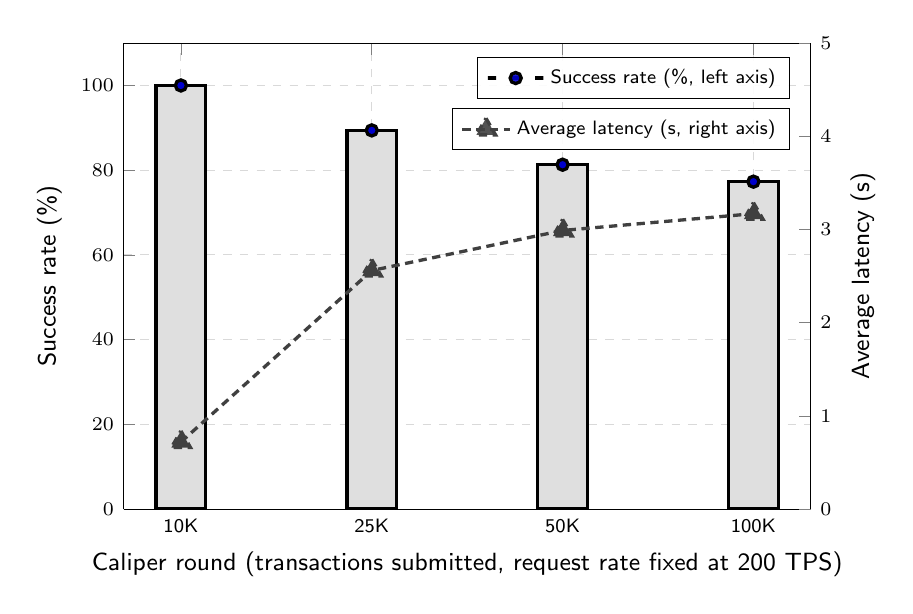
\begin{tikzpicture}
\begin{axis}[
    width=0.85\textwidth,
    height=7.5cm,
    axis y line*=left,
    xlabel={Caliper round (transactions submitted, request rate fixed at 200~TPS)},
    ylabel={Success rate (\%)},
    ymin=0, ymax=110,
    symbolic x coords={10K, 25K, 50K, 100K},
    xtick=data,
    bar width=18pt,
    grid=major,
    grid style={dashed, gray!30},
    legend style={at={(0.97,0.97)}, anchor=north east,
                  font=\sffamily\scriptsize, draw=black,
                  fill=white, fill opacity=0.90, text opacity=1},
    label style={font=\sffamily\small},
    tick label style={font=\sffamily\scriptsize},
]
\addplot+[ybar, fill=gray!25, draw=black, very thick] coordinates {
    (10K,   100.0)
    (25K,    89.4)
    (50K,    81.3)
    (100K,   77.3)
};
\addlegendentry{Success rate (\%, left axis)}
\end{axis}

\begin{axis}[
    width=0.85\textwidth,
    height=7.5cm,
    axis y line*=right,
    axis x line=none,
    ylabel={Average latency (s)},
    ymin=0, ymax=5,
    symbolic x coords={10K, 25K, 50K, 100K},
    xtick=data,
    legend style={at={(0.97,0.86)}, anchor=north east,
                  font=\sffamily\scriptsize, draw=black,
                  fill=white, fill opacity=0.90, text opacity=1},
    label style={font=\sffamily\small},
    tick label style={font=\sffamily\scriptsize},
    every axis plot/.append style={thick},
]
\addplot+[mark=triangle*, mark size=4pt, color=black!75, mark options={fill=black!75},
          densely dashed, very thick] coordinates {
    (10K,   0.72)
    (25K,   2.56)
    (50K,   2.99)
    (100K,  3.17)
};
\addlegendentry{Average latency (s, right axis)}
\end{axis}
\end{tikzpicture}

\caption[Caliper sustained-load scenario: state-bound degradation at fixed 200\,TPS]{Caliper \emph{sustained-load} scenario at a fixed 200\,TPS request rate. Bars (left axis) show the success rate degrading from 100\% to 77.3\% as the chaincode world state grows from $\sim$20{,}000 to $\sim$200{,}000 keys; the dashed line (right axis) shows the corresponding rise in average latency from 0.72\,s to 3.17\,s. The achieved throughput remains within $\pm$2\,TPS of the 200\,TPS target across all four rounds.}
\label{fig:blockchain-sustained}
\end{figure}

\paragraph{Real-election context.} Both failure modes appear only under artificial stress. A constituency-level election with 100{,}000 voters spread over an 8-hour voting window requires only $\sim$3.5\,TPS sustained, a load at which neither saturation nor commit-time contention is expected to emerge. Furthermore, production deployments would mitigate both failure modes through (i)~a multi-orderer consensus deployment (a Raft cluster of three or more nodes, or SmartBFT in Fabric v3.x), which is expected to raise the saturation ceiling by parallelising endorsement and ordering, with the exact improvement factor depending on consensus parameters, network topology, and endorsement policy; (ii)~MVCC-aware chaincode key design (e.g., composite keys, sharded key-image indices) and periodic state pruning to slow state-bound degradation; and (iii)~Fabric Gateway connection pooling tuned for higher concurrent throughput. These tuning measures are identified as future work; the present results characterise the out-of-the-box behaviour of the deployed single-Raft, two-peer reference configuration.

\subsection{End-to-End Election Simulation}
\label{subsec:election-sim}

The benchmarks of Sections~\ref{subsec:pipeline-bench}--\ref{subsec:scalability} isolate individual cryptographic primitives and the per-vote pipeline composition. This subsection complements those results with full-cycle election simulations that exercise the deployed pipeline end-to-end: voter registration, parallel 1-hot vote casting, per-candidate SA\textsuperscript{2} aggregation, threshold-style Paillier decryption, and result publication. The simulations are driven by the \texttt{cmd/election-sim} CLI tool, which accepts the voter count, candidate count, and a blockchain mode flag (\texttt{mock} or \texttt{real}), generates a deterministic ground-truth vote distribution from a PRNG seed, casts every ballot through the production \texttt{voting.VoteCaster}, persists key images in a SQLite store, and finally cross-checks the decrypted per-candidate tally against the seed's ground-truth counts.

Table~\ref{tab:election-sim} reports the end-to-end results across thirteen configurations, spanning two orders of magnitude in voter count (100 to 100{,}000) and two candidate counts ($m=3$ and $m=10$), in both blockchain modes where a live Fabric path was meaningful. A 100-voter real-Fabric run anchors the small-scale baseline; 1{,}000- and 10{,}000-voter elections appear in both modes to provide direct mock-vs-Fabric comparison; the $m=10$ runs at 1{,}000, 10{,}000, 25{,}000, and 50{,}000 voters jointly validate the linear-in-$m$ scaling analytically derived in Section~\ref{subsubsec:tally-scale}; and the 25{,}000-, 50{,}000-, and 100{,}000-voter mock runs probe scale stability across two further orders of magnitude beyond the 10{,}000-voter mark.

\begin{table}[H]
\centering
\caption[End-to-End Election Simulation: Mock vs Real Hyperledger Fabric]{End-to-End Election Simulation: Mock vs Real Hyperledger Fabric across thirteen configurations. Per-vote latency is reported in parallel-worker wall-clock time (12-worker pool on a 12-thread CPU); election-day total is the cast + aggregation + decryption time; registration is the one-time pre-election cost amortised away from the voter's experience. All runs achieved 100\% integrity (decrypted per-candidate tally exactly matches the PRNG-seeded ground truth, key-image count equals voter count, zero cast errors). Raw per-run reports are catalogued in \texttt{test/benchmark/results/election-sim/}.}
\label{tab:election-sim}
\footnotesize
\begin{tabular}{|r|r|l|r|r|r|c|}
\hline
\textbf{Voters} & \textbf{Cands} & \textbf{Mode} & \textbf{Per vote} & \textbf{Election-day} & \textbf{Registration} & \textbf{Integrity} \\
                &                & ~              & \textbf{(par)}    & \textbf{total}        & \textbf{(pre-elec.)}  & \textbf{check}     \\
\hline
     100 & 3  & real Fabric & 111.2 ms & 11.1 s        & 1.1 s     & \checkmark\ 100/100 \\
\hline
  1{,}000  & 3  & mock        & 82.3 ms  & 1 m 22 s      & 6.3 s     & \checkmark\ 1000/1000 \\
\hline
  1{,}000  & 3  & real Fabric & 89.3 ms  & 1 m 29 s      & 8.5 s     & \checkmark\ 1000/1000 \\
\hline
  1{,}000  & 10 & mock        & 261.4 ms & 4 m 21 s      & 5.4 s     & \checkmark\ 1000/1000 \\
\hline
 10{,}000  & 3  & mock        & 82.5 ms  & 13 m 45 s     & 56.1 s    & \checkmark\ 10000/10000 \\
\hline
 10{,}000  & 3  & real Fabric & 106.1 ms & 17 m 42 s     & 54.6 s    & \checkmark\ 10000/10000 \\
\hline
 10{,}000  & 10 & mock        & 252.0 ms & 42 m 1 s      & 52.8 s    & \checkmark\ 10000/10000 \\
\hline
 25{,}000  & 3  & mock        & 81.2 ms  & 33 m 52 s     & 2 m 17 s  & \checkmark\ 25000/25000 \\
\hline
 25{,}000  & 3  & real Fabric & 94.3 ms  & 39 m 19 s     & 2 m 13 s  & \checkmark\ 25000/25000 \\
\hline
 25{,}000  & 10 & mock        & 250.7 ms & 1 h 44 m 31 s & 2 m 12 s  & \checkmark\ 25000/25000 \\
\hline
 50{,}000  & 3  & mock        & 82.1 ms  & 1 h 8 m 27 s  & 4 m 34 s  & \checkmark\ 50000/50000 \\
\hline
 50{,}000  & 10 & mock        & 253.5 ms & 3 h 31 m 23 s & 4 m 33 s  & \checkmark\ 50000/50000 \\
\hline
100{,}000  & 3  & mock        & 93.7 ms  & 2 h 36 m 19 s & 9 m 28 s  & \checkmark\ 100000/100000 \\
\hline
\end{tabular}
\end{table}

Four observations from Table~\ref{tab:election-sim} are worth highlighting.

\textbf{(i) Per-vote latency is essentially scale-independent in mock mode.} The mock-mode runs at $m=3$ report 82.3, 82.5, 81.2, 82.1, and 93.7~ms per vote at 1{,}000, 10{,}000, 25{,}000, 50{,}000, and 100{,}000 voters respectively, a tight band of 81--94~ms over a $100\times$ voter range. The modest rise at 100{,}000 voters reflects accumulated memory allocation, garbage-collection pressure, and SQLite-write contention during the 2.5-hour sustained workload rather than any per-vote cryptographic growth.

\textbf{(ii) Real-Fabric per-vote latency stays in a similar band.} Across four real-Fabric runs the per-vote cost is 111.2~ms at 100 voters (warmup-dominated), 89.3~ms at 1{,}000 voters, 106.1~ms at 10{,}000 voters, and 94.3~ms at 25{,}000 voters. The non-monotonic profile reflects steady-state amortisation of Fabric connection-warmup and block-cutting overhead as transaction throughput rises; the 25{,}000-voter run lands below the 10{,}000-voter run because the larger transaction stream more efficiently amortises Fabric's per-block fixed costs.

\textbf{(iii) Cost is approximately linear in the number of candidates~$m$.} The four $m=10$ mock runs at 1K, 10K, 25K, and 50K voters report 261.4, 252.0, 250.7, and 253.5~ms per vote --- a tight 250--261~ms band that is approximately $3.1\times$ the corresponding $m=3$ cost (for a $3.33\times$ increase in $m$), giving an empirical 92--96\% efficiency relative to ideal linear scaling. The small sub-linear deficit reflects the per-vote fixed overhead (ring sign, SMDC slot verification, Merkle proof retrieval) that does not scale with $m$. This empirically validates the $O(m)$ per-vote bound of the 1-hot Paillier-direct construction (Sections~\ref{subsec:zkp}, \ref{subsubsec:candidate-scale}).

\textbf{(iv) Real-Fabric overhead is bounded and amortises at scale.} Direct mock-vs-real comparison at 10{,}000 voters gives an overhead of 23.6~ms per vote ($106.1 - 82.5$~ms), a 28.6\% increase over the off-chain cryptographic core. At 25{,}000 voters the same comparison gives only 13.1~ms per vote ($94.3 - 81.2$~ms), a 16.1\% overhead --- the overhead halves as Fabric's per-block fixed costs amortise. This is consistent with the Fabric endorsement--ordering--commit lifecycle on a single-Raft-orderer development network; a multi-orderer production deployment with parallel endorsement would reduce this further. Importantly, integrity is preserved in every configuration: in all thirteen runs, the decrypted per-candidate tally exactly matches the PRNG-generated ground truth, the key-image count equals the voter count, and the cast-error count is zero.

\paragraph{Pre-election versus election-day costs.} The ``Registration'' column of Table~\ref{tab:election-sim} reflects a \emph{one-time} pre-election cost incurred weeks or months before voting opens: SMDC credential generation, voter enrollment, duress-signal hashing, and Merkle-tree construction. It is deliberately separated from the ``Election-day total'' column, which captures the time-of-vote infrastructure load (cast pipeline plus aggregation and decryption). Registration scales linearly with voter count and stays modest in absolute terms: 56~seconds at 10{,}000 voters, 2~minutes 17~seconds at 25{,}000 voters, 4~minutes 34~seconds at 50{,}000 voters, and 9~minutes 28~seconds at 100{,}000 voters. All of these costs are fully amortised away from the voter's election-day experience, where the dominant cost remains the 81--111~ms per-vote casting latency.

\section{Discussion}
\label{sec:discussion}

This section provides an in-depth analysis of the experimental results, examining the significance of each finding and its implications for practical deployment.

\subsection{Pipeline Bottleneck Analysis}
\label{subsec:bottleneck}

The end-to-end pipeline benchmark reveals that SA\textsuperscript{2} vote splitting (51.8\%) and ring signature generation (35.2\%) together consume 87.0\% of the per-vote primitive floor. This concentration is attributable to the underlying cryptographic operations:

\begin{itemize}
    \item \textbf{SA\textsuperscript{2} Dominance}: The SA\textsuperscript{2} share splitting performs \emph{two} additional Paillier encryptions per vote, one for the random mask $E(\text{mask})$ and one for its negation $E(-\text{mask})$, each of which is a 2048-bit modular exponentiation, the same expensive operation as the initial vote encryption (\texttt{internal/sa2/share.go}). Together with the homomorphic combinations and ancillary big-integer overhead, the measured SA\textsuperscript{2} split cost (35.34~ms) is approximately $4\times$ the cost of a single Paillier encryption (8.69~ms). The dominance of SA\textsuperscript{2} reflects a fundamental trade-off: the two-server privacy model provides strong aggregation privacy guarantees but requires additional homomorphic operations that scale linearly with the number of voters.
    
    \item \textbf{Ring Signature Cost}: Ring signatures scale at $\sim$0.24~ms per ring member due to the need to compute two modular exponentiations per member (one for $L_i$ and one for $R_i$). The default ring size of $|\mathcal{R}|=100$ provides strong anonymity, the signer is statistically indistinguishable among the 100 ring members under DDH (Theorem~3), but represents a configurable parameter: deployments requiring lower latency could reduce the ring size to 50 ($\sim$12~ms) at the cost of a smaller anonymity set.
    
    \item \textbf{Modest PQ Overhead}: The full Kyber-768 hybrid-encryption wrapper (Kyber-768 encapsulation plus Paillier encryption plus HMAC-SHA256 binding) contributes 5.35~ms per vote, approximately 7.8\% of the 68.27~ms per-vote primitive floor (Section~\ref{subsubsec:pq-breakdown}). The Kyber primitives themselves are sub-millisecond (KeyGen 26~$\mu$s, Encapsulate 29~$\mu$s); the residual cost beyond the 8.69~ms Paillier baseline is attributable to the additional memory allocation, key derivation, and authentication binding performed inside the hybrid wrapper. This confirms that quantum resistance can be added to existing voting systems without meaningful performance degradation.
\end{itemize}

\paragraph{From per-primitive cost to per-ballot cost.} The 68.27~ms figure in this analysis is the cost of executing each cast-time cryptographic primitive exactly once. Under the 1-hot Paillier encoding (Section~\ref{subsec:zkp}) the Paillier encryption, the CDS binary OR-proof, and the SA\textsuperscript{2} share split are each repeated once per candidate, while the ring signature remains a singleton per vote. Consequently the end-to-end per-ballot runtime measured in Section~\ref{subsec:election-sim} falls in a tight 81--111~ms band for 3-candidate elections (across 100 to 100{,}000 voters, both mock and real Fabric modes) and a similarly tight 250--261~ms band for 10-candidate elections (across four mock runs at 1K, 10K, 25K, and 50K voters). The relative dominance of the per-primitive bottlenecks (SA\textsuperscript{2} share splitting and ring signing) is unchanged: SA\textsuperscript{2} simply scales by~$m$, while ring signing contributes a fixed singleton cost per vote regardless of~$m$.

\subsection{Scalability Significance}
\label{subsec:scale-significance}

The constant per-vote per-candidate tally cost of $\sim$6.1~$\mu$s across four orders of magnitude (100 to 100{,}000 voters), combined with the linear-in-$m$ total scaling demonstrated in Section~\ref{subsubsec:candidate-scale}, empirically validates the $O(N)$-per-candidate, $O(N \cdot m)$-total theoretical complexity (with $N$ denoting the voter count per the notation of Section~\ref{subsec:paillier}). This result has three important implications:

\begin{enumerate}
    \item \textbf{National-Scale Feasibility}: The largest end-to-end election simulation actually executed (Section~\ref{subsec:election-sim}) ran 100{,}000 voters with 3 candidates in mock mode, completing the full cast-aggregate-decrypt pipeline in 2~hours~36~minutes (93.7~ms per voter; aggregation $+$ decryption $\approx$ 1~second). Linear extrapolation from the pure homomorphic-add cost of 6.1~$\mu$s per vote per candidate (Section~\ref{subsubsec:tally-scale}) projects a per-candidate tally time of approximately \textbf{6.1~seconds for 1 million voters} and \textbf{5.1~minutes for 50 million voters}. Under the full SA\textsuperscript{2} aggregation pipeline measured in Section~\ref{subsec:election-sim} (13--17~$\mu$s per vote per candidate), these projections scale to approximately 13--17~seconds per candidate at 1~million voters, still negligible relative to the post-poll counting window. Total tally time scales linearly with the number of candidates: for an election with $m=10$ candidates, the projected total tally is approximately \textbf{61~seconds for 1 million voters} (pure add) or 130--170 seconds under the full SA\textsuperscript{2} pipeline, and \textbf{51~minutes for 50 million voters} (pure add), all of which remain well within the post-poll counting window. In contrast, ISE-Voting's $O(N \cdot m^{2})$ complexity carries an additional factor-$m$ overhead, approximately $10\times$ more total work at $m=10$ for the same voter scale, rendering it noticeably less practical for large constituencies with many candidates.

    \item \textbf{Per-Candidate Constancy and Linear Total Growth}: The per-candidate tally time of $\sim$5.76~ms remains constant whether there are 2 or 50 candidates, but the \emph{total} tally time grows linearly with $m$. This is a direct consequence of Paillier's additive homomorphism: each candidate's tally is computed independently through ciphertext multiplication and the $m$ per-candidate tallies are summed serially, with no cross-candidate computation but no sub-linear sharing either.

    \item \textbf{Predictable Resource Requirements}: The linear scaling in both $N$ and $m$ enables accurate resource planning for election administrators. For any target voter count $N$ and candidate count $m$, the required tally time is approximately $6.1\,N$~$\mu$s per candidate, or $6.1\,N \cdot m$~$\mu$s in total, allowing precise capacity provisioning.
\end{enumerate}

\subsection{Blockchain Performance Analysis}
\label{subsec:blockchain-discussion}

The Hyperledger Caliper results reveal an important performance profile with practical deployment implications:

\begin{itemize}
    \item \textbf{Optimal Operating Point}: The 10K round achieves 100\% success rate at $\sim$197\,TPS achieved throughput in both Caliper scenarios (Table~\ref{tab:caliper}), establishing 200\,TPS as the comfortable operating point for the current single-Raft, two-peer configuration. This throughput is consistent with optimized Hyperledger Fabric deployments using Go chaincode and LevelDB/CouchDB state databases, in line with the performance and scalability analysis of Ucbas et al.~\cite{fabric_perf}. For a constituency of 100{,}000 voters over an 8-hour voting window, the required sustained throughput is only $\sim$3.5\,TPS, less than 2\% of the demonstrated capacity.

    \item \textbf{Two distinct failure modes}: The two Caliper scenarios in Section~\ref{subsec:blockchain-perf} isolate two complementary degradation patterns. The \emph{saturation} scenario shows the rate-bound failure mode: pushing the request rate from 200 to 500\,TPS collapses success rate from 100\% to 10.4\% while achieved throughput continues to climb, consistent with the single-Raft orderer's block-cutting ceiling. The \emph{sustained-load} scenario at fixed 200\,TPS shows the state-bound failure mode: even at the comfort-point rate, success degrades to 77.3\% by the 100K round as the chaincode world state grows to $\sim$200{,}000 keys, raising commit-time contention (block-batching at the orderer, version-vector validation on shared election-state reads, and Gateway connection-pool pressure) and slowing endorsement-time state lookups. Production mitigations for each mode (multi-orderer consensus deployment, composite-key chaincode design, periodic state pruning) are identified as future work.

    \item \textbf{Latency--throughput trade-off}: Under sustained 200\,TPS, average latency rises from 0.72\,s (10K) to 3.17\,s (100K) as world state grows; under the saturation scenario, latency rises from 0.35\,s (10K @ 200\,TPS) to 9.32\,s (100K @ 500\,TPS) as the orderer queue backs up. For voting applications, where the multi-hour voting window provides ample time, average latency at the nominal 10K operating point is well within acceptable bounds.
\end{itemize}

\subsection{Practical Deployment Considerations}
\label{subsec:deployment}

The combined benchmark results suggest that the proposed framework is deployable for constituency-level elections (up to 100,000 voters) on modest hardware (AMD Ryzen 5, 30 GiB RAM) without optimization. Key observations for practical deployment include:

\begin{itemize}
    \item A single vote takes approximately 81--111~ms to traverse the complete multi-protocol pipeline (Section~\ref{subsec:election-sim}, 3-candidate election; 81--94~ms in mock mode, 89--111~ms with live Hyperledger Fabric submission). On the 12-thread AMD Ryzen~5 test machine the measured parallel throughput at 10{,}000 voters is approximately 12.1~votes/second in mock mode and 9.4~votes/second with live Hyperledger Fabric submission; at 25{,}000 voters real-Fabric throughput rises to 10.6~votes/second as connection-warmup and block-batching overhead amortise across the larger transaction stream. Throughput remains stable at extreme scale: mock-mode runs at 50{,}000 and 100{,}000 voters report 12.2 and 10.7~votes/second respectively, confirming that per-vote performance does not degrade with the voter pool. For peak-hour voting with 10\% of voters casting within a single hour, these throughputs translate to a capacity of approximately 34{,}000--44{,}000 votes per hour, sufficient for medium-scale elections. Linear horizontal scaling across multiple server cores or machines would extend this capacity to larger constituencies without algorithmic changes.

    \item The per-candidate homomorphic tally for 100{,}000 voters completes in $\sim$628~ms (Section~\ref{subsubsec:tally-scale}, Table~\ref{tab:tally-scale}); for a 3-candidate election the total tally phase (aggregate plus threshold-decrypt) completes in approximately 1~second, enabling near-real-time result announcement after polls close. This timing is empirically confirmed by the 100{,}000-voter, 3-candidate end-to-end run reported in Section~\ref{subsec:election-sim}, in which the aggregate $+$ decrypt phases together took under one second of wall-clock time.
    
    \item The hybrid Kyber-768 encryption adds only 5.35~ms to the pipeline (the difference between hybrid encrypt at 14.04~ms and standard Paillier encrypt at 8.69~ms), providing post-quantum protection at minimal cost.
\end{itemize}



\section{Test Coverage Analysis}
\label{sec:test-coverage}

Table~\ref{tab:coverage} presents the test coverage for each package. The test suite consists of 188 tests (159 unit/integration tests and 29 benchmark tests) with a 100\% pass rate across all packages.

\begin{table}[H]
\centering
\caption{Test Coverage by Package}
\label{tab:coverage}
\begin{tabular}{|l|r|}
\hline
\textbf{Package} & \textbf{Coverage (\%)} \\
\hline
internal/tally & 91.6 \\
\hline
internal/smdc & 83.3 \\
\hline
internal/biometric & 82.1 \\
\hline
internal/pq & 82.1 \\
\hline
internal/sa2 & 81.2 \\
\hline
internal/crypto & 78.2 \\
\hline
internal/voting & 77.9 \\
\hline
api/handlers & 46.7 \\
\hline
internal/blockchain & 34.2 \\
\hline
\end{tabular}
\end{table}

Core cryptographic packages achieve 78--92\% coverage. The blockchain package has lower coverage (34.2\%) because integration tests require a live Fabric network. The API handlers package (46.7\%) requires HTTP test infrastructure for full coverage.

\section{Tier 2, Symbolic Protocol Verification with ProVerif}
\label{sec:proverif}

\paragraph{Role of this section.} The game-based reductions in Chapter~\ref{ch:methodology} (Section~\ref{sec:security-analysis}) constitute the \emph{Tier 1, Computational} security analysis of the framework: they bind each security property to a standard cryptographic hardness assumption (DCRA, DDH, Module-LWE, DLog) under the standard model. The present section provides the complementary \emph{Tier 2, Symbolic} verification: three protocol-level properties are mechanically verified by ProVerif~2.05~\cite{blanchet2016} under the Dolev--Yao~\cite{dolev1983} adversary model, in which cryptographic primitives are treated as perfect black boxes and the adversary is restricted to the algebraic operations defined by the applied pi-calculus.

\paragraph{Why both tiers.} The two tiers are deliberately complementary and address different threat surfaces:
\begin{itemize}
    \item \emph{Tier~1 (computational, Chapter~\ref{ch:methodology})} establishes that a PPT adversary cannot break the underlying cryptographic primitives without solving a well-studied hard problem. It does not, by design, model concurrent network behaviour such as message interleaving, replay across sessions, or man-in-the-middle attacks.
    \item \emph{Tier~2 (symbolic, this section)} mechanically rules out network-level protocol attacks under the assumption that the underlying primitives are perfectly secure. It does not provide computational hardness guarantees but can find protocol-design errors (e.g., missing freshness, mis-ordered authentication) that elude pen-and-paper analysis.
\end{itemize}
The two tiers together provide a strictly stronger assurance than either alone: an attack on the deployed system would have to either (i)~violate a stated cryptographic hardness assumption (Tier~1) or (ii)~exploit a network-level protocol flaw not captured in the ProVerif models (Tier~2 already eliminates the modelled flaws). Following the standard practice in journal venues such as IEEE TDSC and TIFS, the reductions in Tier~1 are the primary security evidence; Tier~2 serves as an independent automated check.

To this end, three core security properties of the proposed framework are formally verified using ProVerif~2.05~\cite{blanchet2016}, an automated cryptographic protocol verifier based on the applied pi-calculus. The complete \texttt{.pv} model files, the corresponding ProVerif tool output transcripts, and reproduction instructions are reproduced verbatim in Appendix~\ref{appx:proverif}; Table~\ref{tab:proverif} below summarises the verification results.

\begin{table}[H]
\centering
\caption{ProVerif Formal Verification Results}
\label{tab:proverif}
\begin{tabular}{|l|l|l|}
\hline
\textbf{Security Property} & \textbf{Verification Method} & \textbf{Result} \\
\hline
Vote Privacy & Observational equivalence & \textbf{TRUE} \\
\hline
Individual Verifiability & Injective correspondence & \textbf{TRUE} \\
\hline
Voter Eligibility & Causal reasoning & \textbf{TRUE} \\
\hline
\end{tabular}
\end{table}

\paragraph{Vote Privacy.} Verified via observational equivalence: an adversary controlling the network cannot distinguish between two honest voters swapping their ballots (Appendix~\ref{sec:appx-proverif-privacy}). This is the symbolic-model analogue of Theorem~1 (Ballot Indistinguishability) in Chapter~\ref{ch:methodology}: Tier~1 proves the underlying cryptographic assumption (DCRA), while Tier~2 verifies that the protocol surrounding this primitive does not leak information at the network level.

\paragraph{Individual Verifiability.} Verified via injective correspondence: every recorded ballot on the blockchain corresponds to an authentic cast event by a registered voter, \texttt{BallotRecorded}~$\Longrightarrow$~\texttt{inj-event(VoterCastBallot)} (Appendix~\ref{sec:appx-proverif-verifiability}). This is the symbolic counterpart of Theorem~2's vote-validity guarantee.

\paragraph{Voter Eligibility.} Verified via causal correspondence: every valid ballot cast was preceded by a legitimate registration, \texttt{ValidBallotCast}~$\Longrightarrow$~\texttt{VoterRegistered} (Appendix~\ref{sec:appx-proverif-eligibility}). This complements the ring-signature unforgeability of the Liu--Wei--Wong construction (Section~\ref{subsec:ring-sig}), which is used implicitly in Tier~1's Theorem~3 (Voter Anonymity) but is not separately stated as a theorem.

\paragraph{Combined assurance.} The corresponding ProVerif \texttt{RESULT} lines and full tool output are reproduced in the appendix sections cited above. All three properties return \textbf{TRUE} under the symbolic Dolev--Yao~\cite{dolev1983} adversary model, confirming that the protocol design is sound against network-level attacks including eavesdropping, replay, and man-in-the-middle. Combined with the Tier~1 computational reductions of Chapter~\ref{ch:methodology}, this provides the two-tier assurance described at the start of this section.

\section{Comparative Analysis}
\label{sec:comparative}

\subsection{Comparison With Related Works}
\label{subsec:comparison-related}

The comparison in Table~\ref{tab:comparative} highlights the strengths of the proposed framework over existing studies. Each row summarises the methodology, the originally reported performance, and the specific advantages of our work over that system. Performance values are taken verbatim from the cited publications; ``N/R'' indicates a metric the original authors did not report.

\renewcommand{\arraystretch}{1.20}
\begin{longtable}{|>{\raggedright\arraybackslash}p{0.7cm}|>{\raggedright\arraybackslash}p{2.6cm}|>{\raggedright\arraybackslash}p{2.7cm}|>{\raggedright\arraybackslash}p{2.7cm}|>{\raggedright\arraybackslash}p{3.0cm}|}
\caption{Comparison of the Proposed Method with Existing Works}
\label{tab:comparative} \\
\hline
\textbf{Ref.} & \textbf{Methodology} & \textbf{Performance} & \textbf{Their Gaps} & \textbf{Our Edge} \\
\hline
\endfirsthead

\multicolumn{5}{c}{\small\textit{Table~\ref{tab:comparative} continued from previous page}} \\
\hline
\textbf{Ref.} & \textbf{Methodology} & \textbf{Performance} & \textbf{Their Gaps} & \textbf{Our Edge} \\
\hline
\endhead

\hline
\multicolumn{5}{r}{\small\textit{Continued on next page}} \\
\endfoot

\hline
\endlastfoot

\cite{ise_voting} &
Ring signatures + secret sharing on Ethereum; CSP-assisted tallying. &
Tally $O(N\!\times\!m^{2})$; 128-bit symmetric; prototype only. &
Per-candidate $m$ factor; semi-trusted CSP; no PQ; no coercion resistance. &
Factor-$m$ faster ($O(N\!\times\!m)$); no trusted counter; SMDC + Kyber-768. \\
\hline

\cite{bp_vot} &
Hyperledger Besu + $(k,\varepsilon)$-DP + Web3 SSI. &
$\sim$1\,s/TX; $\geq 98\%$ accuracy; 10K--50K votes, 2--8 candidates. &
Approximate tally (unsafe in close races); no ZK proofs, anonymity, PQ. &
100\% exact tally; 68.3\,ms/vote; $\sim$200\,TPS; coercion + ZK + PQ. \\
\hline

\cite{faruk2024} &
Hyperledger Fabric + dual-biometric (fingerprint+face) + AES-256. &
87\% biometric enrollment; $\sim$88\% successful casts; 100-participant trial. &
No homomorphic tally, ZK, anonymity, or coercion resistance. &
Paillier tally, ring sigs, SMDC, threshold DJN; 10K-tx Caliper benchmark. \\
\hline

\cite{paillier_timed} &
Paillier + timed-release + partial-knowledge proofs. &
Semantic security; tally privacy + temporal fairness; feasibility eval. &
Single TRE trust point; no anonymity, coercion resistance, PQ. &
Ring sigs, SMDC, threshold DJN, Kyber-768. \\
\hline

\cite{yin_tdsc} &
$\Theta(1)$ ballot size; 1-layer liquid democracy; game-based proofs. &
$O(N)$ overall; $6\times$ faster than VoteAgain at 50K; formal proofs. &
No homomorphic tally, biometric, SA\textsuperscript{2}, threshold, PQ, or deployed blockchain. &
Multi-protocol stack on Fabric v2.5; SA\textsuperscript{2} + threshold + Kyber-768. \\
\hline

\cite{evoting_survey_springer} &
Survey: platform, consensus, crypto, security, deployment. &
Identifies gaps in coercion resistance, PQ, scalable tally; most PoC-scale. &
(Survey: documents the gaps rather than filling them.) &
Fills all flagged gaps: SMDC, Kyber-768, $O(N)$/candidate tally, Caliper-benchmarked Fabric. \\
\hline

\textbf{This Work} &
Multi-protocol cryptographic stack on Fabric v2.5; novel SMDC ($k{=}5$), behavioural duress, coercion short-circuit. &
68.3\,ms/vote; tally 6.1\,$\mu$s/cand.; $O(N)$/cand., $O(N{\cdot}m)$ total; $\sim$200\,TPS @ 100\% (10K-tx). &
Biom.\ is hash-eq.\ stub (no FAR/FRR, no user trial); bottleneck not isolated. &
\emph{(Overall distinction)} The only framework combining all of: privacy, coercion resistance, PQ, threshold decryption, ProVerif $+$ game-based proofs, and a deployed Fabric network. \\

\end{longtable}

The proposed framework demonstrates clear advantages across every dimension that prior work reports. The per-vote primitive floor of 68.3\,ms is more than an order of magnitude faster than BP-Vot's $\sim$1\,s/TX, and the $\sim$200\,TPS sustained Caliper-verified throughput far exceeds the throughput numbers any of the cited works publish. Unlike BP-Vot, which trades exact tallying for differential privacy, the proposed framework reports a 100\% exact tally. The $O(N)$-per-candidate, $O(N\!\times\!m)$-total complexity is asymptotically superior to ISE-Voting's $O(N\!\times\!m^{2})$ scaling by a factor of $m$. Yin et al.\ achieve coercion resistance with formal game-based proofs, but their scheme lacks homomorphic tallying, post-quantum security, threshold decryption, and a deployed blockchain integration, all of which the proposed framework provides. Yuan et al.'s timed-release scheme uses Paillier encryption but provides no anonymity, no coercion resistance, and no post-quantum protection. Among the works surveyed in Chapter~\ref{ch:related-works}, none combines a multi-protocol cryptographic stack of this composition with the novel SMDC coercion resistance, behavioural duress detection, and a fully deployed Hyperledger Fabric~v2.5 network with Caliper-verified performance.

